%
% General structure for the revdetua class:
%
\documentclass{revdetua}
%
% Valid options are:
%
%   longpaper --------- \part and \tableofcontents defined
%   shortpaper -------- \part and \tableofcontents not defined (default)
%
%   english ----------- main language is English (default)
%   portugues --------- main language is Portuguese
%
%   draft ------------- draft version
%   final ------------- final version (default)
%
%   times ------------- use times (postscript) fonts for text
%
%   mirror ------------ prints a mirror image of the paper (with dvips)
%
%   visiblelabels ----- \SL, \SN, \SP, \EL, \EN, etc. defined
%   invisiblelabels --- \SL, \SN, \SP, \EL, \EN, etc. not defined (default)
%
% Note: the final version should use the times fonts
% Note: the really final version should also use the mirror option
%
\usepackage{graphicx}
\usepackage{subfig}
\usepackage{appendix}
\usepackage{tabularray}

\begin{document}

\Header{98012}{1}{novembro}{2022}{1}
% Note: the month must be in Portuguese

\title{Algoritmos de Pesquisa Exaustiva \& Greedy Heuristic para encontrar\newline um conjunto dominante com k vértices de um grafo}
\author{Gonçalo Freitas \\Mestrado em Engenharia Computacional} % or \author{... \and ...}
\maketitle

\begin{abstract}% Note: in English
Given a undirected graph G(V, E), use an exhaustive search and a greedy heuristic approach to find if the graph as a dominating set with k vertices. An analysis about the computational complexity, time execution and number of basic operations of the problem will also be made.
\end{abstract}

\begin{resumo}% Note: in Portuguese
Dado um grafo não direcionado G(V, E), é usado um algoritmo de pesquisa exaustiva e um algoritmo heurístico para descobrir se o grafo têm um conjunto dominante com k vértices. Também será feita uma análise sobre a complexidade computacional, o tempo de execução e o número de operações básicas do problema. 
\end{resumo}

%\begin{keywords}% Note: in English (optional)
 % ...
%\end{keywords}

\begin{palavraschave}% Note: in Portuguese (optional)
Grafos, Conjunto Dominante, Complexidade Computacional, Pesquisa Exaustiva, Greedy Heuristic
\end{palavraschave}

\section{Introdução}

\subsection{Conjunto Dominante}
\label{Teoria_Grafos}
Na teoria dos grafos, um conjunto dominante de um grafo $G$, com $V$ vértices e $E$ arestas, $G = (V, E)$, é um subconjunto $D$ de $V$ de tal forma que cada vértice que não está em $D$ é adjacente a pelo menos um membro de $D$.


\begin{figure}[h!]
\centering
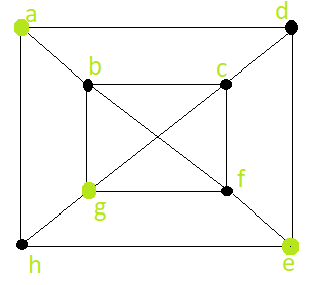
\includegraphics[scale = 1.0]{Figs/DominatingSET.png}
\caption{Exemplo de um grafo com 8 vértices com conjunto dominante.\cite{Dominating}}
\label{DSET}
\end{figure}

Analisando o grafo da Fig.\ref{DSET} podemos afirmar que um conjunto dominante deste grafo poderá ser $D = \{a, g, e\}$.

Posto isto, o principal objetivo de ambos os algoritmos é encontrar, se possível, um conjunto dominante com $K \times V$ vértices, onde $K$ corresponde a uma percentagem do número total de vértices, $V$. Para este problema iremos considerar $K \in [0.125, 0.25, 0.50, 0.75]$. Contudo, como o resultado de $K \times V$ podem não ser um valor inteiro irá ser usada a função $math.floor$ de forma a obter o número inteiro igual ou inferior ao resultado desta operação.

\subsection{Pesquisa Exaustiva}
A pesquisa exaustiva baseia-se numa abordagem de força bruta, geralmente aplicada a problemas combinatórios, cuja estratégia pode ser descrita pelos seguintes passos.\cite{Slides}
\begin{enumerate}
\label{enum:features}
    \item[1.] Enumerar todos os candidatos para a solução
    \item[2.] Verificar se satisfazem as condições do problema
    \item[3.] Se necessário, escolher uma solução do conjunto de candidatos viáveis (que são solução)
\end{enumerate}

Neste caso, apenas queremos saber se existe algum conjunto dominante de $K$ vértices, não quantos existem. Uma melhor explicação do algoritmo encontra-se em \ref{Al_Ex}. 

\subsection{Greedy Heuristic}
Um Greedy Heuristic algortihtm é uma abordagem para resolver um problema através da seleção da melhor opção disponível no momento, não se preocupando se esta seleção levará ao melhor resultado global. O algoritmo nunca inverte a decisão anterior, mesmo que a esta seleção esteja errada. Funciona numa abordagem 'top-down'.\cite{programiz}

Este algoritmo pode não produzir o melhor resultado para todos os problemas mas, quando consegue, geralmente tem uma performance melhor. Outra vantagem destes algoritmos é a maior facilidade de descrever o algoritmo. Uma melhor explicação do algoritmo desenvolvido encontra-se em \ref{Al_GH}. 

\section{Algoritmos}
\subsection{Pesquisa Exaustiva}
\label{Al_Ex}
No nosso caso, para implementar este algoritmo, começamos por gerar todas as combinações de vértices possíveis. Por exemplo, para $V = 3$, as combinações possíveis seriam:
\[
[(0), (1), (2), (0, 1), (0, 2), (1, 2), (0, 1, 2)]
\]

Contundo, assumindo que, por exemplo, $K = 0.50$, as soluções possíveis seriam apenas:
\[
[(0), (1), (2)]
\]

No código, de maneira a tornar o algoritmo mais eficiente, esta lista com os conjuntos candidatos a solução não é guardada mas sim calculada a cada iteração pois, à medida que o tamanho do grafo aumenta o número de conjuntos aumenta, pelo que, guardar a lista tornaria-se muito penalizador em termos de memória e rapidez.

Após ter uma lista com os conjuntos que podem ser solução basta iterar e procurar se existe algum conjunto que verifica as condições de conjunto dominante. Caso não exista nenhum é retornado um conjunto vazio. Caso exista, o código retorna imediatamente esse conjunto e finaliza a execução.

\subsection{Greedy Heuristic}
\label{Al_GH}

Quanto ao Greedy Heuristic, este algoritmo pode ser realizado de várias maneiras, dependendo de como se decide abordar o problema. Após uma análise de vários grafos gerados pelo package NetworkX e fazendo uso da função dominating\_set(G), foi possível observar que o vértice 0 faz parte de um dos conjuntos dominantes aproximadamente 90\% das vezes. Posto isto, decidiu-se seguir uma abordagem em que, apenas se vai analisar os conjuntos em que esteja presente o vértice 0. Assim, analisando o exemplo demonstrado em \ref{Al_Ex} só existira um conjunto possível de ser solução, o conjunto (0).

Posto isto, este código é bastante semelhante aquele da pesquisa exaustiva apenas com a adição da condição de que o vértice 0 tem que fazer parte dos conjuntos a analisar, o que, por sua vez, diminui o número de conjuntos candidatos a solução e torna o algoritmo menos exigente em termos computacionais, como iremos ver mais a frente.

%Pesquisa Exaustiva vista anteriormente mas diminuindo ainda mais o número de soluções possíveis pois apenas serão consideradas aquelas que respeitam as condições já impostas mais uma nova condição, possuir o vértice 0 no conjunto


\section{Análise}
A package NetworkX permite-nos gerar um grafo aleatório com $V$ vértices e atribuir a uma aresta uma certa probabilidade, $P$, de ela existir. Para este problema iremos considerar $V \in [4, 5, 6, ..., 25]$ e $P \in [0.125, 0.25, 0.50, 0.75]$. Os valores de $K$ considerados serão aqueles já referidos na introdução.



\subsection{Análise Formal}
\label{AnlForm}

O problema apresentado retrata-se num tradicional problema resolvido por um método de pesquisa exaustiva de verificar, de todas as combinações de $n$ vértices do grafo, com tamanho $k$, quais satisfazem a condição. O número de combinações de $n$ vértices com tamanho $k$ pode ser traduzido no seguinte somatório:

\[
\sum\limits_{k=1}^{n \choose k} 1
\]

Dado uma combinação, de forma a verificar se se traduz num conjunto dominante, é necessário verificar todos os vértices que não estão na combinação e todos que se encontram na combinação. No total temos $n-k$ vértices que não pertencem à combinação, o que se traduz num somatório de $j=1$ até $n-k$. Por outro lado, temos $k$ vértices que pertencem a combinação, o que leva a um somatório de $g=1$ até $k$. Assim sendo, esta verificação é traduzida em dois somatórios como os de seguida:

\[
\sum\limits_{j=1}^{n-k}\sum\limits_{g=1}^{k} 1 
\]

Juntando os 3 somatórios apresentados temos:

\[
\sum\limits_{k=1}^{n \choose k}\sum\limits_{j=1}^{n-k}\sum\limits_{g=1}^{k} 1 = k(n-k){n \choose k} = k(n-k) \frac{n!}{k! (n-k)!}
\]

Simplificando vem, 
\[
k(n-k) \frac{n!}{k! (n-k)!} = n!\frac{k}{k(k-1)!}\frac{(n-k)}{(n-k)(n-k-1)!} =
\]
\[
=\frac{1}{k(k-1)!}\frac{n!}{(n-k-1)!} 
\]

Como  $n!$ cresce mais rapidamente do que $(n-k-1)!$ podemos então concluir que este problema possui uma complexidade computacional $n!$, $\mathcal{O}(n!)$, onde $\mathcal{O}$ representa a notação de \textit{Big-O}.

Não foi possível realizar um fit fatorial aos nossos dados com o programa Matlab contudo, analisando as curvas representadas na Fig.\ref{fit}, podemos confirmar que os nossos dados seguem uma distribuição do tipo $a\times (n-b)! + c$, o que nos ajuda a confirmar a complexidade computacional obtida através da análise formal realizada anteriormente.

\begin{figure}[h!]
\centering
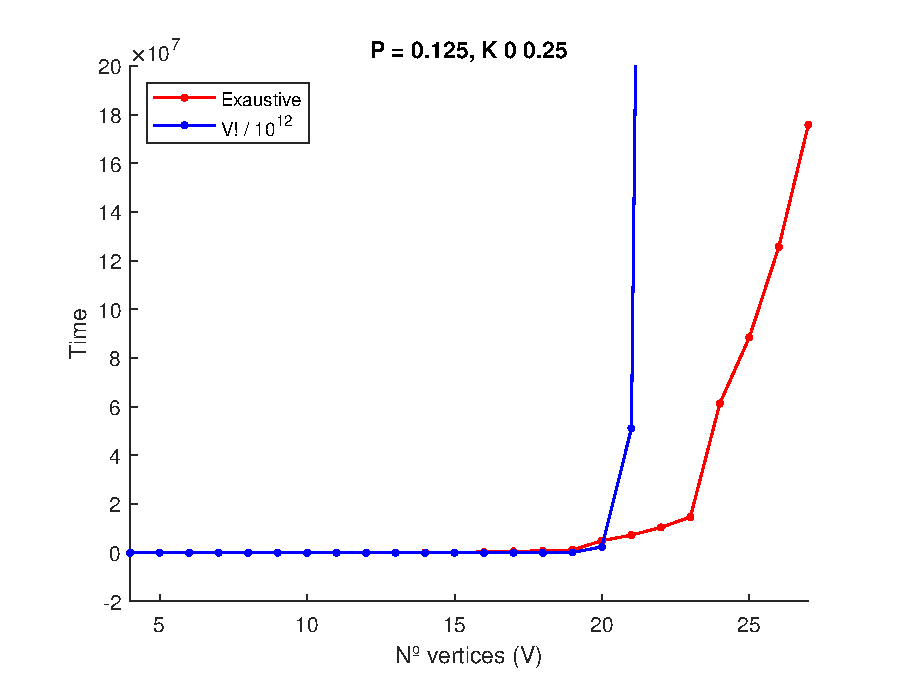
\includegraphics[scale = 0.5]{Figs/try_fit.eps}
\caption{Comparação do tempo de execução do algoritmo exaustivo com $V!$, em função de V}
\label{fit}
\end{figure}

\subsection{Resultados}

\subsubsection{Exemplos}

Na Fig.\ref{graf_example} podemos ver um exemplo de um grafo gerado pela package NetworkX, para valores de $V = 6$, $K = 0.50$, $P = 0.75$. Neste exemplo, ambos os algoritmos retornaram, como resposta, o conjunto \{0,1,2\}. Com base no explicado em \ref{Teoria_Grafos}, podemos concluir que este é realmente um conjunto dominante e com o tamanho pretendido ($math.floor(K\times V)$).

\begin{figure}[h!]
\centering
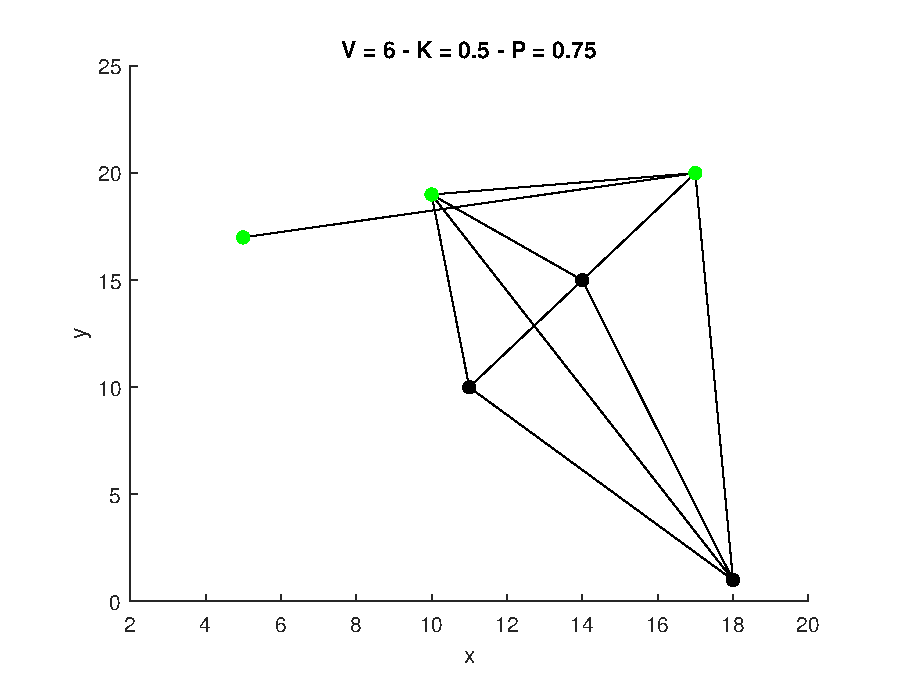
\includegraphics[scale = 0.5]{Figs/example_graph.eps}
\caption{Exemplo de um grafo gerado fazendo uso da package NetworkX, para  $V = 6$, $K = 0.50$, $P = 0.75$, onde ambos os algoritmos encontraram solução}
\label{graf_example}
\end{figure}

Já nas Figuras \ref{graf_example1} e \ref{graf_example2} podemos ver os outros dois casos, isto é, quando apenas o algoritmo Exaustivo e quando nenhum encontra uma solução de tamanho pretendido, respetivamente.

\begin{figure}[h!]
\centering
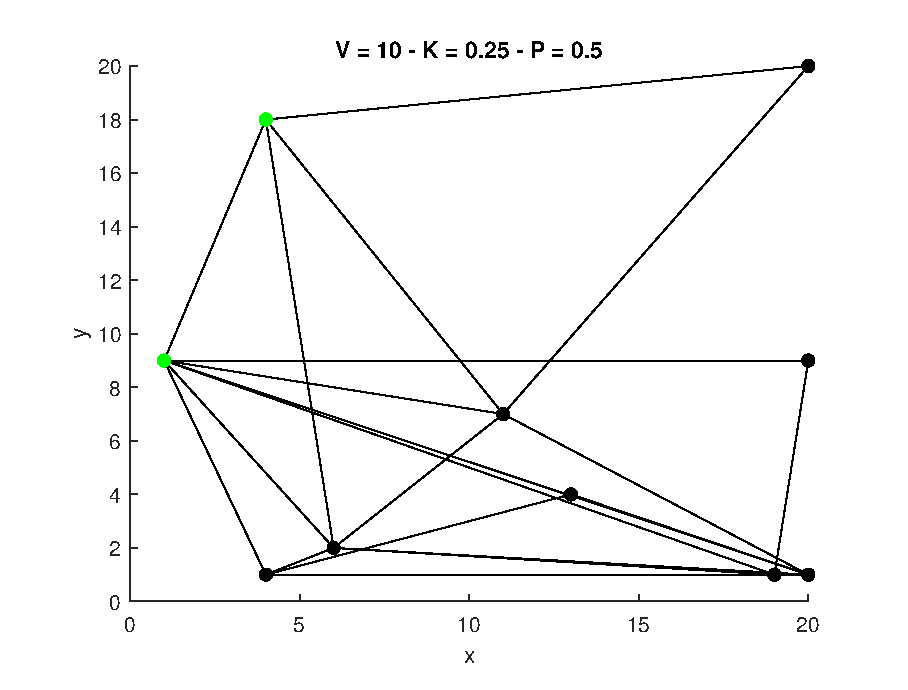
\includegraphics[scale = 0.5]{Figs/example_graph_Exaust.eps}
\caption{Exemplo de um grafo gerado fazendo uso da package NetworkX, para  $V = 6$, $K = 0.25$, $P = 0.5$, onde apenas o algoritmo Exaustivo encontrou solução}
\label{graf_example1}
\end{figure}

\begin{figure}[h!]
\centering
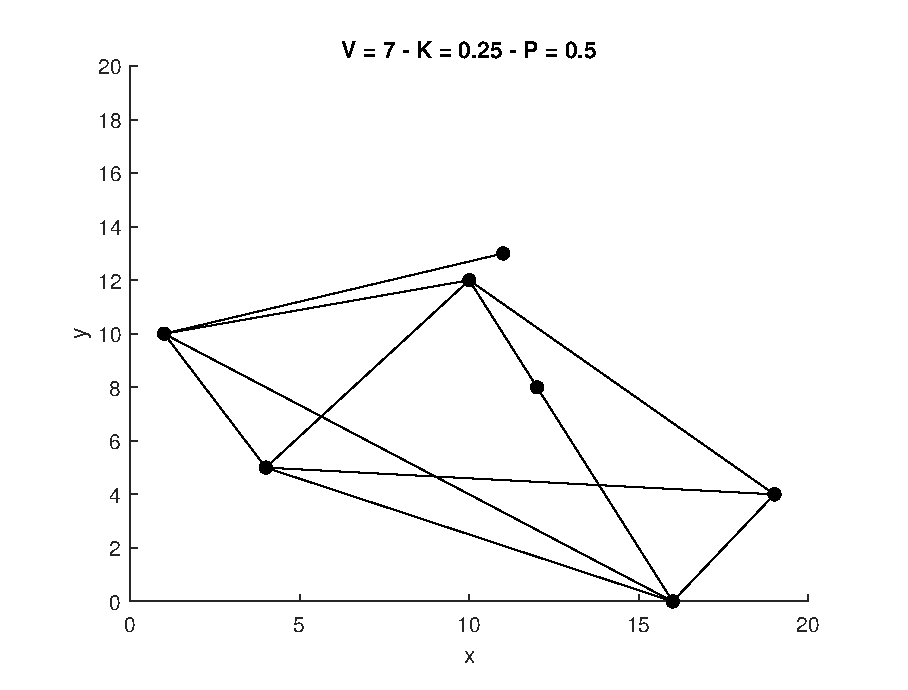
\includegraphics[scale = 0.5]{Figs/example_graph_None.eps}
\caption{Exemplo de um grafo gerado fazendo uso da package NetworkX, para  $V = 7$, $K = 0.25$, $P = 0.5$, onde nenhum algoritmo encontrou solução}
\label{graf_example2}
\end{figure}

Após uma análise de 'papel e caneta' foi possível confirmar que no exemplo da Figura \ref{graf_example1} não existe nenhuma solução que cumpra os requisitos do algoritmo Heurístico, isto é, o vértice 0 pertencer ao conjunto dominante e o conjunto ter tamanho 2. Já no exemplo da Figura \ref{graf_example2} foi possível confirmar que não existe nenhuma solução possível de tamanho 1, o que nos dá mais certeza que os algoritmos estão a funcionar corretamente.

\subsubsection{$P = 0.125$}

Para os outros valores de P os gráficos representativos aos tempos de execução e ao número de operações de cada algoritmo encontram-se no Appendix \ref{APP_RES}. Estes não foram alvo de análise pois esta seria igual a que será feita para um valor de $P = 0.125$.

\begin{figure}[h!]
\centering
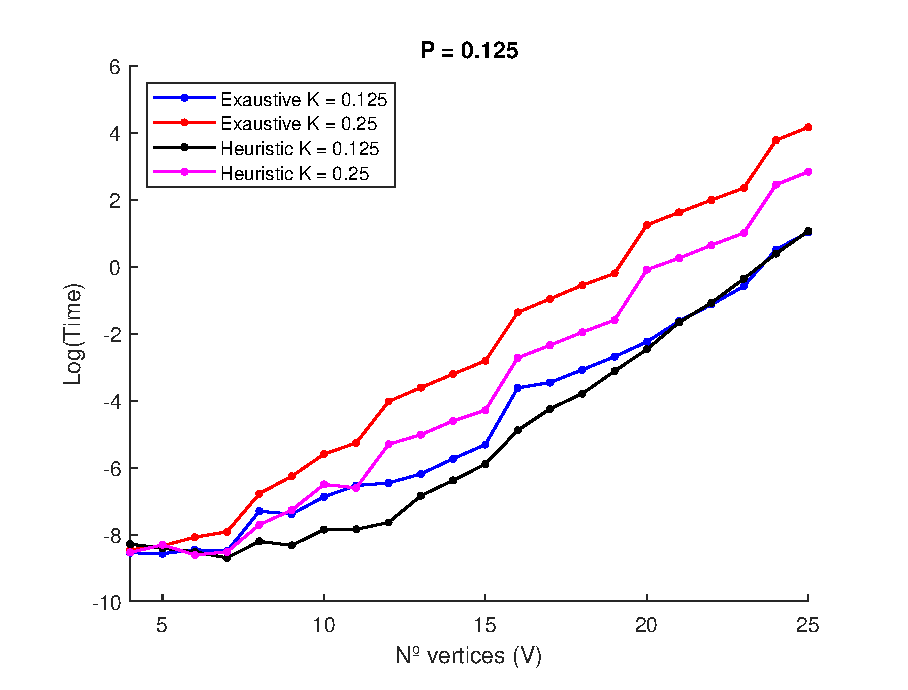
\includegraphics[scale = 0.5]{Figs/1_P0125.eps}
\caption{Logaritmo do tempo de execução dos algoritmos em função do número de vértices - $P = 0.125$ - $K = 0.125, 0.25$}
\label{1_P0125}
\end{figure}


\begin{figure}[h!]
\centering
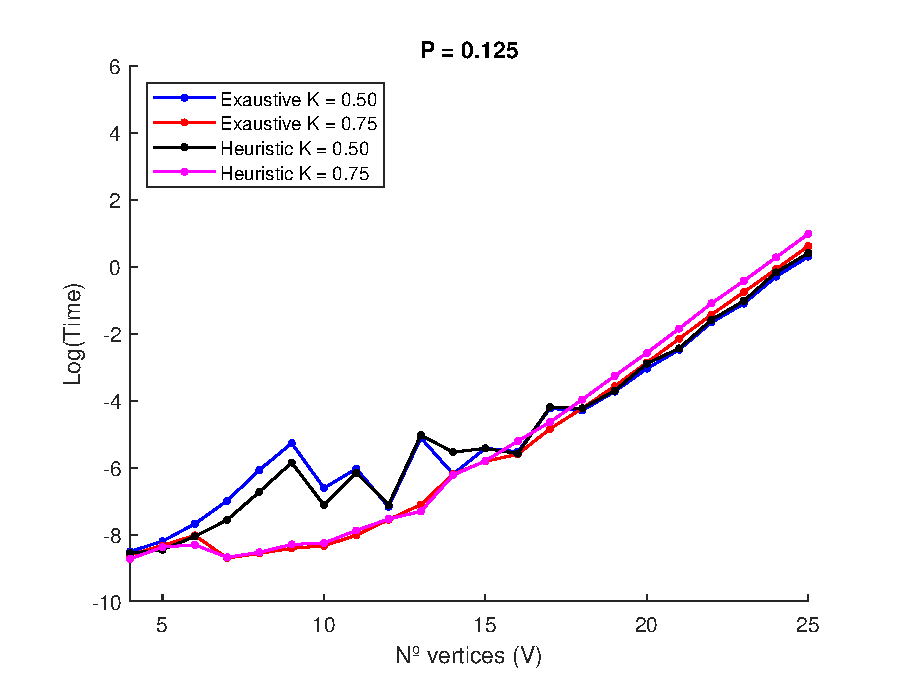
\includegraphics[scale = 0.5]{Figs/2_P0125.eps}
\caption{Logaritmo do tempo de execução dos algoritmos em função do número de vértices - $P = 0.125$ - $K = 0.50, 0.75$}
\label{2_P0125}
\end{figure}

Analisando primeiramente os tempos de execução reparamos que, tal como esperado, estes crescem de uma maneira exponencial, como se pode ver pelas Fig.\ref{1_P0125} e Fig.\ref{2_P0125}. Reparamos também que o algoritmo Heurístico apresenta quase sempre melhores tempos. Foi feito uma análise mais profunda para perceber quando isto não acontecia e foi descoberto que apenas acontece quando o algoritmo Heurístico não funciona, isto é, quando o algoritmo de pesquisa Exaustiva encontra um conjunto dominante mas o Heurístico não.
No entanto, o tempo de execução não é a melhor maneira de comparar algoritmos pois este depende de vários fatores e pode induzir em erro. No entanto, uma boa maneira de comparar algoritmos é comparar o número de operações básicas que cada algoritmo realiza. 

\begin{figure}[h!]
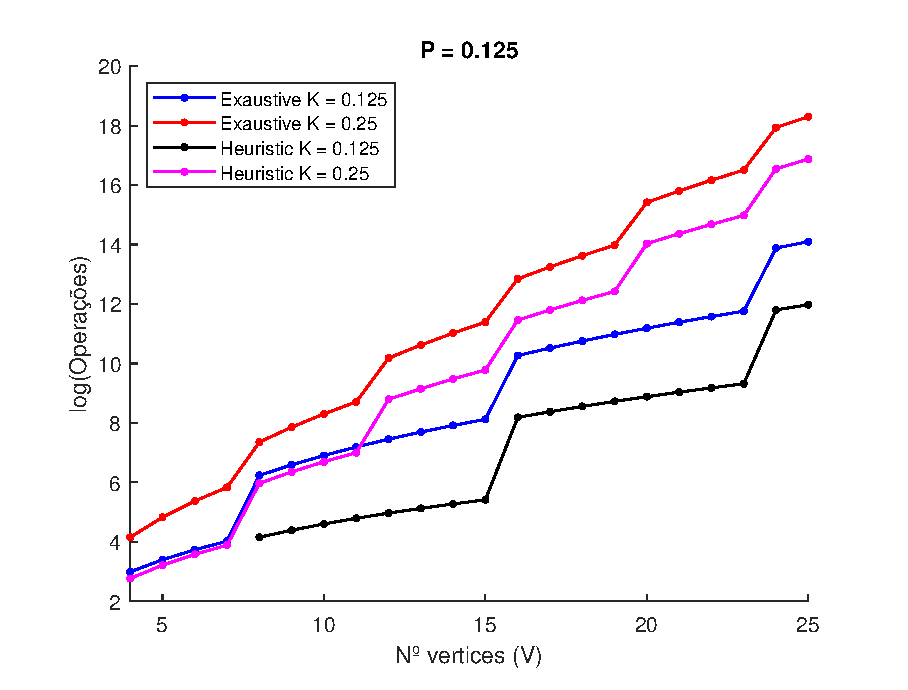
\includegraphics[scale = 0.5]{Figs/3_P0125.eps}
\caption{Logaritmo do número de operações realizadas pelos algoritmos em função do número de vértices - $P = 0.125$ - $K = 0.125, 0.25$}
\label{3_P0125}
\end{figure}

\begin{figure}[h!]
\centering
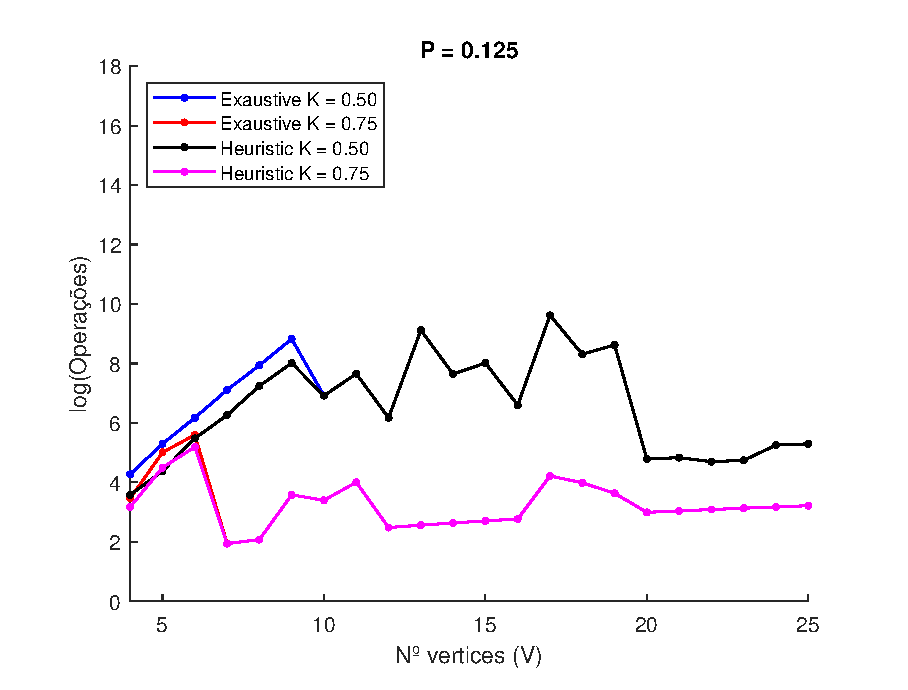
\includegraphics[scale = 0.5]{Figs/4_P0125.eps}
\caption{Logaritmo do número de operações realizadas pelos algoritmos em função do número de vértices - $P = 0.125$ - $K = 0.50, 0.75$}
\label{4_P0125}
\end{figure}

Analisando então o número de operações realizadas por cada algoritmo para cada valor de $K$ e para grafos de vários tamanho, Fig. \ref{3_P0125} e \ref{4_P0125}, rapidamente reparamos que o algoritmo Exaustivo realiza mais ou o mesmo número de operações mas nunca menos que o algoritmo Heurístico. Isto permite-nos concluir, tal como esperado, que o algoritmo Heurístico traz vantagens no estudo deste problema.

%\subsubsection{$P = 0.50$}
%\subsubsection{$P = 0.25$}
%\subsubsection{$P=0.125$}

\subsection{Número de configurações}

Também poderíamos estudar o número de configurações testadas, isto é, o número de conjuntos testados até encontrar uma solução ou chegar ao fim. Contudo, este número seria proporcional ao número de comparações, já analisado anteriormente, Fig.\ref{3_P0125} e \ref{4_P0125}, e que podemos confirmar pelas Fig.\ref{Conf_1_P0125} e \ref{Conf_2_P0125} que realmente o são.

\begin{figure}[h!]
\centering
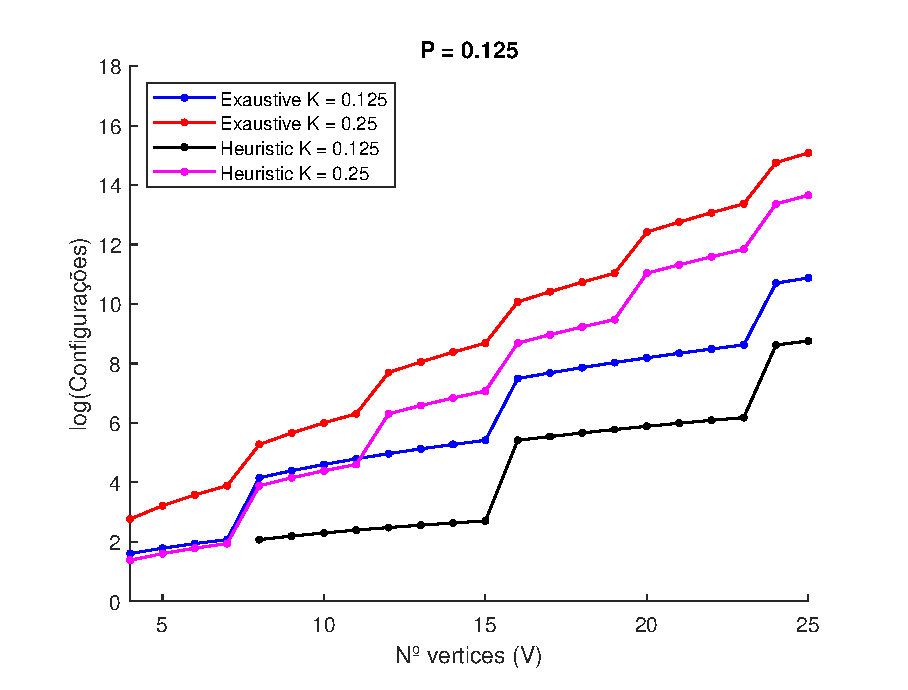
\includegraphics[scale = 0.5]{Figs/Conf_1_P0125.eps}
\caption{Logaritmo do número de configurações testadas pelos algoritmos em função do número de vértices - $P = 0.125$ - $K = 0.125, 0.25$}
\label{Conf_1_P0125}
\end{figure}

\begin{figure}[h!]
\centering
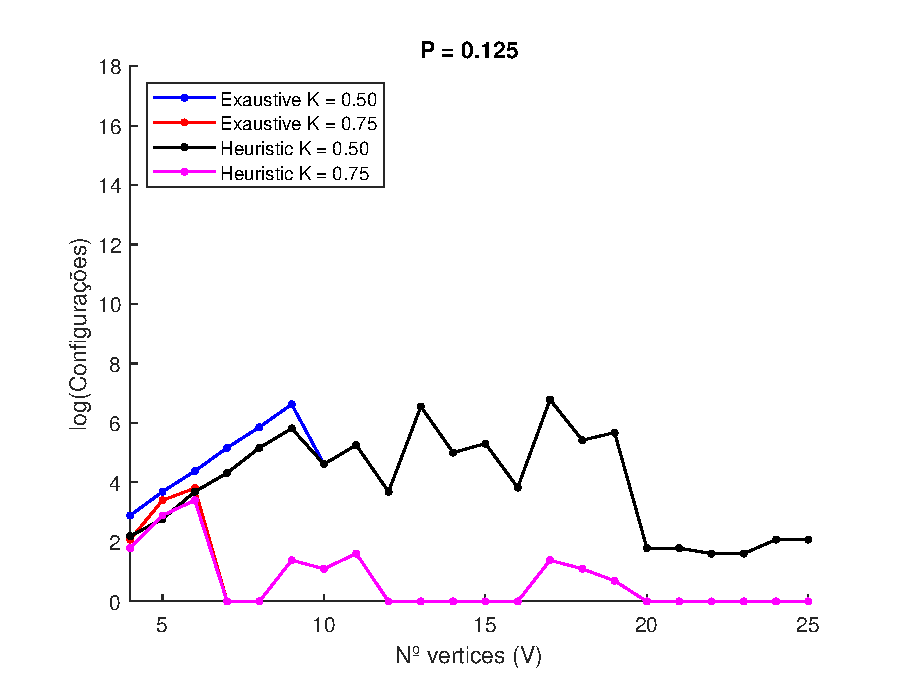
\includegraphics[scale = 0.5]{Figs/Conf_2_P0125.eps}
\caption{Logaritmo do número de configurações testadas pelos algoritmos em função do número de vértices - $P = 0.125$ - $K = 0.50, 0.75$}
\label{Conf_2_P0125}
\end{figure}

\subsection{Grafos de dimensões maiores}

Como o tempo de execução cresce de forma exponencial e o número de operações de forma $n!$, resolver este problema, para grafos de grandes dimensões, exigiria um grande poder computacional e demoraria um grande período de tempo. No entanto, podemos estimar quanto tempo um problema de dimensão $N$ demoraria. Para isso, basta usar os nossos dados e realizar uma extrapolação (exponencial) destes de forma a obter uma estimativa do tempo pretendido.

O máximo número de vértices calculado foi de $V = 30$ (embora apenas tenha sido feito uma análise até $V = 25$). Em média, o algoritmo Exaustivo tem um tempo de execução de  aproximadamente 6 minutos por par $(K,P)$, para $V = 30$. Já para o algoritmo Heurístico este tempo médio é de aproximadamente 2 minutos. Assumindo $P = 0.125$, $K = [0.125, 0.25, 0.5, 0.75]$ e $V \in [4,5,...,30]$ no total, isto é, $Time_{exaustive} + Time_{hueristic}$, foi preciso um tempo de execução de aproximadamente 53 minutos. Vamos apenas considerar $P = 0.125$ e $K = 0.25$ para estudar o tempo necessário para grafos de dimensões maiores, visto que para outros valores de $P$ e de $K$ o procedimento seria o mesmo.

\begin{figure}[h!]
\centering
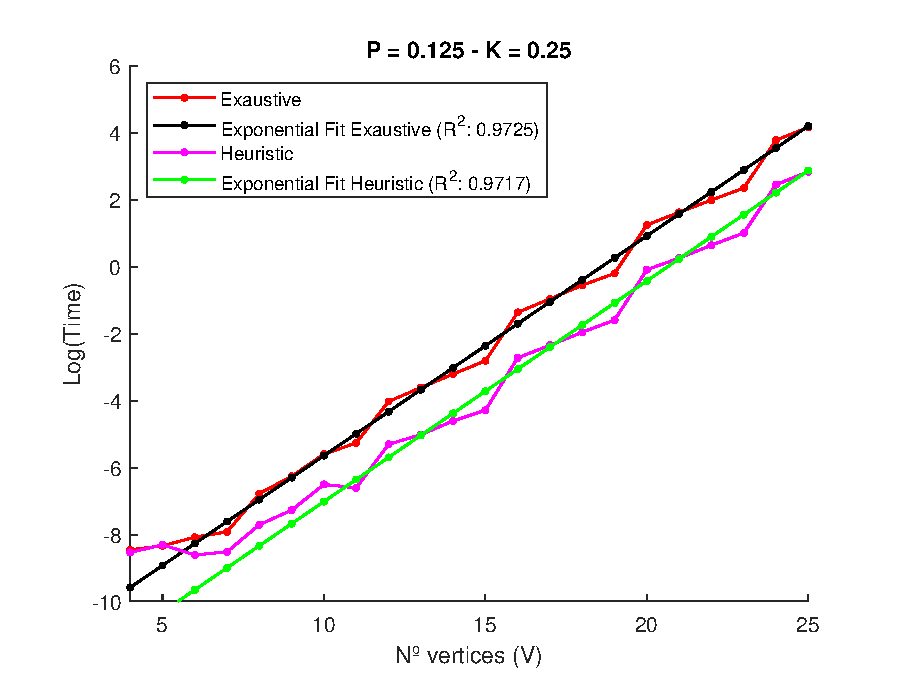
\includegraphics[scale = 0.5]{Figs/extrapol.eps}
\caption{Logaritmo do número de configurações testadas pelos algoritmos em função do número de vértices + Exponential Fits - $P = 0.125$ - $K = 0.25$}
\label{extrapol}
\end{figure}

Na Fig.\ref{extrapol} estão representados os fits realizados aos dados do algoritmo Exaustivo e do algoritmo Heurístico, cujas equação são as seguintes, respetivamente:

\[
    f(x) = (4.992\times 10^{-6})  \times e^{0.6566x}
\]
\[
    f(x) = (1.226\times 10^{-6}) \times e^{0.6596x}
\]

Podemos então usar estas equações para estimar quanto tempo seria necessário para executar os nossos algoritmos para grafos de tamanho $V = N$, cujos valores se encontram representados na Tabela \ref{extr}, para alguns valores de $N$.


\begin{table}[h!]
\centering
\small
\caption{Estimativas do tempo de execução dos algoritmos para $V = N$}
\label{extr}
\begin{tabular}{|c|c|c|c|}
\hline
 $(V, Time(s))$  & $Heuristic$  & $Exaustive$ & $|diff|$\\ \hline
$V = 35$  & $1.3020\times 10^{4}$ & $4.7731\times 10^{4}$ & 3.4711\\ \hline
$V = 40$  & $3.5230\times 10^{5}$ & $1.2723\times 10^{6}$ & 920000\\ \hline
$V = 45$ & $9.5328\times 10^{6}$ & $3.3914\times 10^{7}$ & 24381200\\ \hline
$V = 50$  & $2.5794\times 10^{8}$ &  $9.0399\times 10^{8}$ & 646050000\\ \hline
\end{tabular}
\end{table}

Esta tabela permite-nos também perceber que à medida que o tamanho do grafo aumenta, a diferença entre o tempo de execução dos algoritmos, $diff$, vai aumentando, pelo que, o algoritmo Exaustivo começa a ser menos viável, sendo preferível optar pelo algoritmo Heurístico.

\section{Soluções}

Outra análise que pode ser feita é o número de vezes que o nosso algoritmo Heurístico encontra uma solução, versus o número de vezes que o algoritmo de pesquisa Exaustiva encontra. É de esperar que sempre que o algoritmo Heurístico encontre uma solução o algoritmo Exaustivo também encontre. Isto é exatamente o que acontece como se pode ver comparando as Tabelas \ref{Heursi} e \ref{ExS}, onde vemos que o número de soluções obtidas pelo algoritmo Heurístico, por par $(K,P)$, é sempre menor ou igual ao número de soluções obtidas pelo algoritmo Exaustivo. No Appendix \ref{App_Solut}, podemos ver mais detalhadamente quando é que cada algoritmo encontra uma solução, isto é, para que valor/valores de $V$ é que existe uma solução dado um par $(K,P)$, onde verificamos que o algoritmo Heurístico nunca encontra uma solução para um grafo de certo tamanho sem o algoritmo Exaustivo também encontrar. 
Aqui vamos apenas analisar a diferença de vezes que o algoritmo Heurístico encontra uma solução perante o algoritmo Exaustivo, para $V = [4,5,...,30]$.

\begin{table}[h!]
\caption{Total número de soluções encontradas para o algoritmo Heurístico}
\label{Heursi}
\small
\centering
\begin{tabular}{|c|c|c|c|c|c|}
\hline
 $(K,P)$  & $P = 0.125$  & $P = 0.25$  & $P = 0.50$ & $P = 0.75$  \\ \hline
$K = 0.125$  & 0 & 0 & 7 & 15 \\ \hline
$K = 0.25$  & 0 & 14 & 20 & 23 \\ \hline
$K = 0.50$ & 21 & 24 &  27 & 27\\ \hline
$K = 0.75$  & 24 &  25 & 27 & 27\\ \hline
Total & 45 &  63 &  81 & 92 \\ \hline
\end{tabular}
\end{table}

\begin{table}[h!]
\caption{Total número de soluções encontradas para o algoritmo de Pesquisa Exaustiva}
\label{ExS}
\small
\centering
\begin{tabular}{|c|c|c|c|c|c|}
\hline
 $(K,P)$  & $P = 0.125$  & $P = 0.25$  & $P = 0.50$ & $P = 0.75$  \\ \hline
$K = 0.125$  & 0 & 0 & 15 & 23 \\ \hline
$K = 0.25$  & 2 & 14 & 22 & 27 \\ \hline
$K = 0.50$ & 21 & 24 &  27 & 27\\ \hline
$K = 0.75$  & 24 &  26 & 27 & 27\\ \hline
Total & 47 &  74 &  91 & 104 \\ \hline
\end{tabular}
\end{table}

Sabendo que no máximo, por conjunto de $(K,P)$, temos 27 soluções, comparando o número de soluções encontradas pelos algoritmos vemos que, em média, o algoritmo Heurístico encontra 89.58\% do número de soluções do algoritmo Exaustivo, pelo que podemos concluir que o algoritmo Heurístico desenvolvido é uma boa proposta de abordagem ao problema. Em relação ao número total de soluções possíveis vemos que, em média, o algoritmo Heurístico encontra um conjunto dominante 65.05\% das vezes enquanto que o algoritmo Exaustivo encontra 73.15 \% das vezes.

\section{Aplicações na vida real}

Grafos são objeto de vários estudos e têm inúmeras aplicações na vida real como, redes sociais, redes biológicas, recomendações de produtos, mapas/gps entre muitas outras,\cite{AppGraphs}. Para este problema em específico, uma boa aplicação seria, por exemplo, junto da polícia para descobrir os chefes por detrás de uma rede criminosa, isto pois, os chefes contactam com vários trabalhadores que, em principio, têm pouco contacto entre sim, ou seja, dado N suspeitos e as suas relações poderíamos estudar o conjunto dominante para encontrar quem estaria por detrás da rede criminosa. %Outra aplicação seria em redes wireless para encontrar rotas eficientes.

\section{Conclusão}

Este trabalho permitiu por em prática vários tópicos, desde os mais teóricos, como a análise formal para descobrir a complexidade computacional, aos mais práticos, nomeadamente a escrita de código.

Foi possível também reparar nas vantagens e desvantagens dos algoritmos Heurísticos, em que vimos que é possível obter uma solução correta mais rapidamente mas no entanto também pode não ser obtida nenhuma solução, apesar desta existir.

Quanto a pesquisa Exaustiva é possível concluir que, apesar de ser um algoritmo de fácil escrita e compreensão, para casos de dimensões maiores não é uma opção viável devido a ser um algoritmo que requer um grande poder computacional devido à sua grande complexidade.


%\bibliography{...} % use a field named url or \url{} for URLs
% Note: the \bibliographystyle is set automatically
\bibliography{ref.bib}
\printbibliography



\clearpage
\appendix

\section{Análise - Resultados}
\label{APP_RES}


\begin{figure}[h!]
\centering
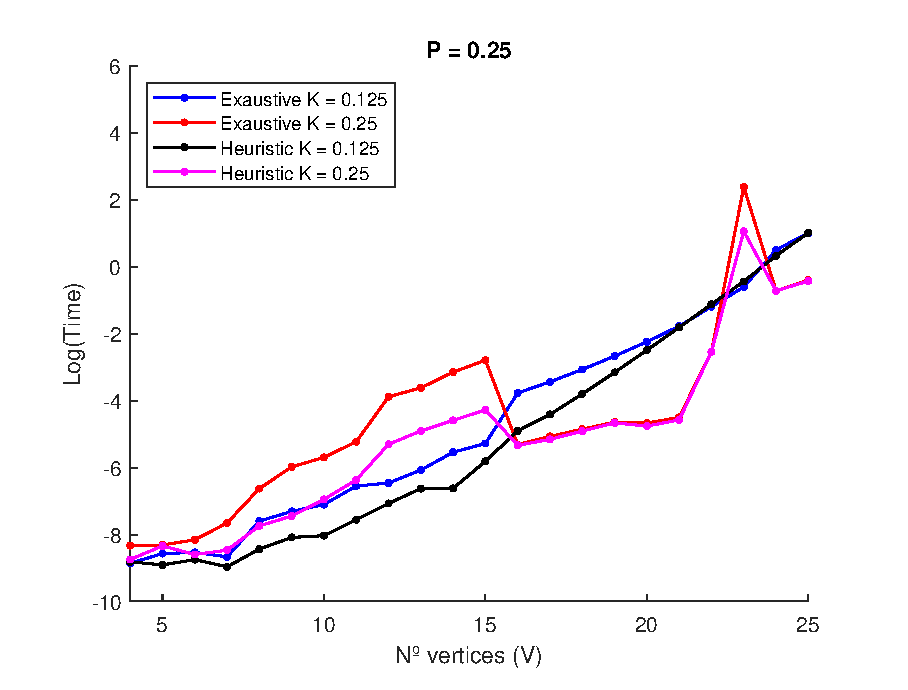
\includegraphics[scale = 0.5]{Figs/1_P025.eps}
\caption{Logaritmo do tempo de execução dos algoritmos em função do número de vértices - $P = 0.25$ - $K = 0.125, 0.25$}
\label{1_P025}
\end{figure}

\begin{figure}[h!]
\centering
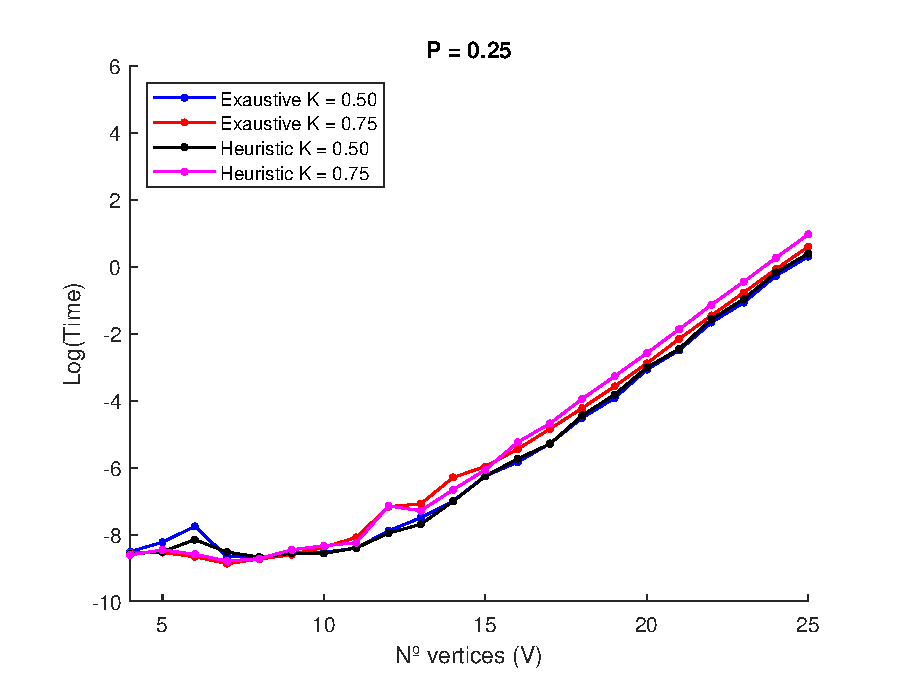
\includegraphics[scale = 0.5]{Figs/2_P025.eps}
\caption{Logaritmo do tempo de execução do algoritmo Exaustivo em função do número de vértices - $P = 0.25$ - $K = 0.50, 0.75$}
\label{2_P025}
\end{figure}

\begin{figure}[h!]
\centering
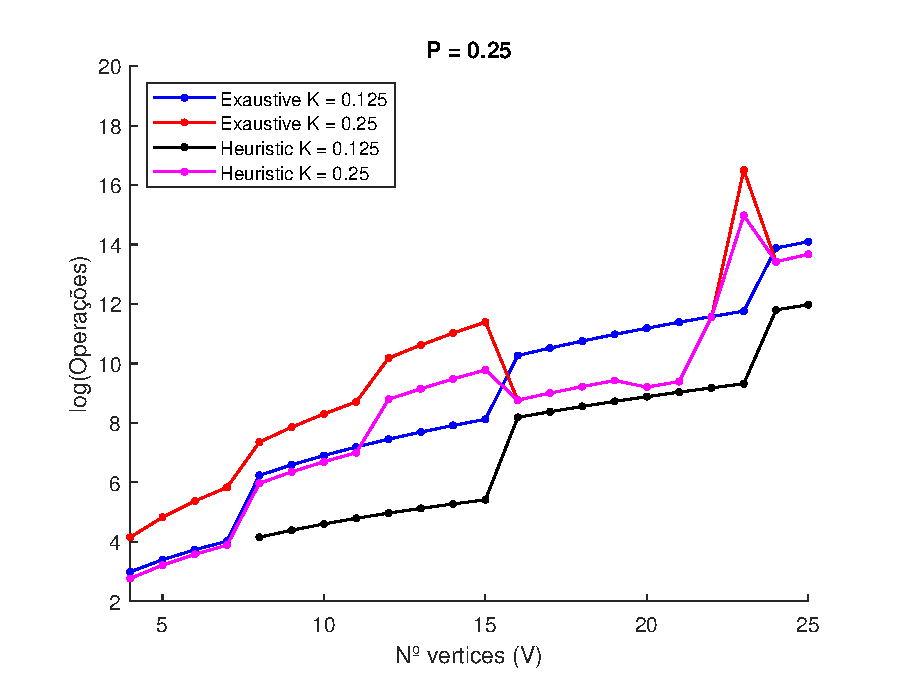
\includegraphics[scale = 0.5]{Figs/3_P025.eps}
\caption{Logaritmo do número de operações realizadas pelos algoritmos em função do número de vértices - $P = 0.75$ - $K = 0.125, 0.25$}
\label{3_P025}
\end{figure}

\begin{figure}[h!]
\centering
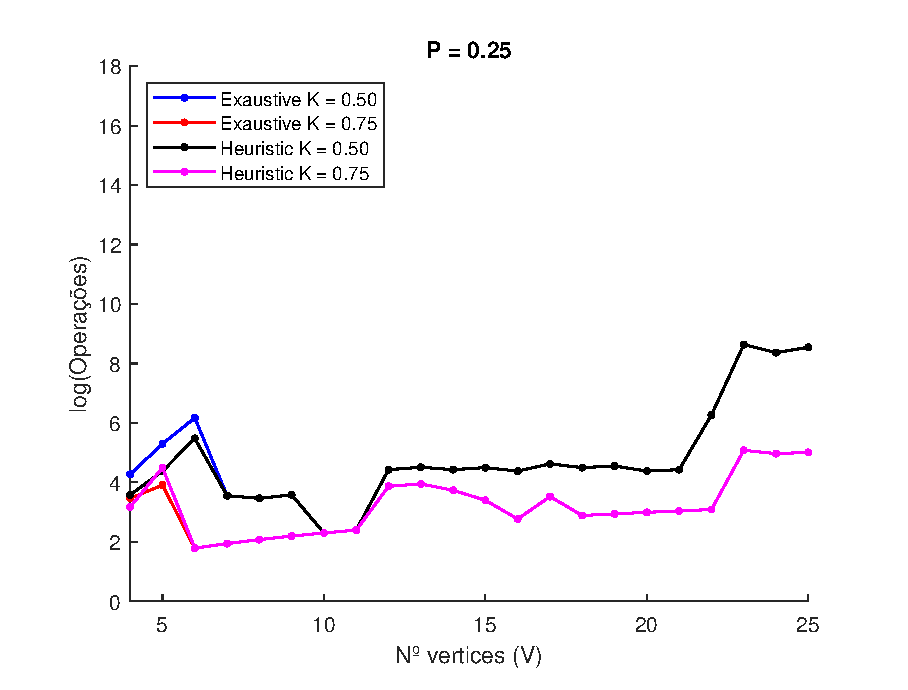
\includegraphics[scale = 0.5]{Figs/4_P025.eps}
\caption{Logaritmo do número de operações realizadas pelos algoritmos em função do número de vértices - $P = 0.25$ - $K = 0.50, 0.75$}
\label{4_P025}
\end{figure}


\begin{figure}[h!]
\centering
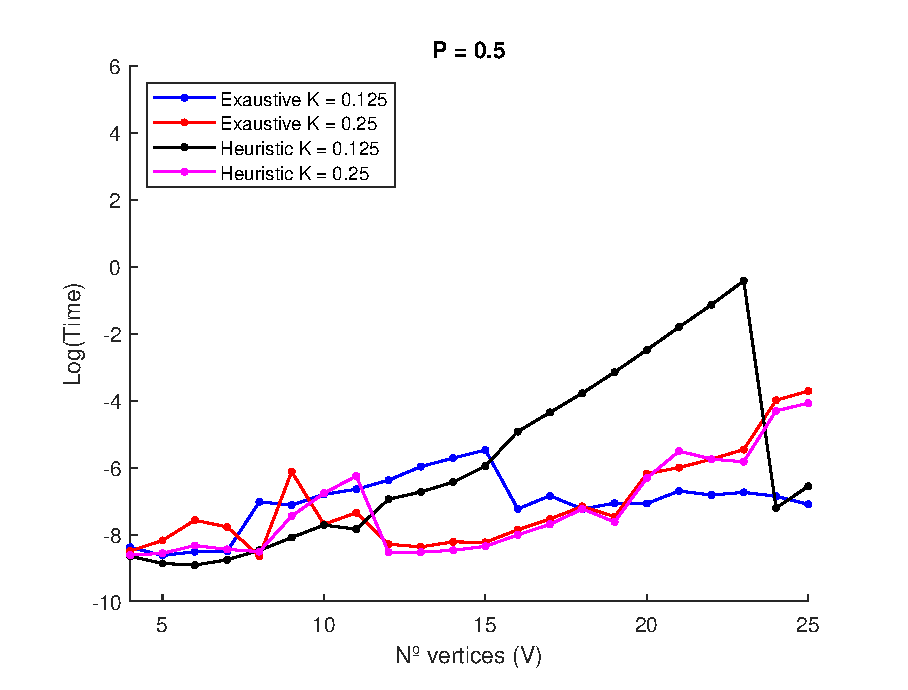
\includegraphics[scale = 0.5]{Figs/1_P050.eps}
\caption{Logaritmo do tempo de execução dos algoritmos em função do número de vértices - $P = 0.25$ - $K = 0.125, 0.25$}
\label{1_P050}
\end{figure}

\begin{figure}[h!]
\centering
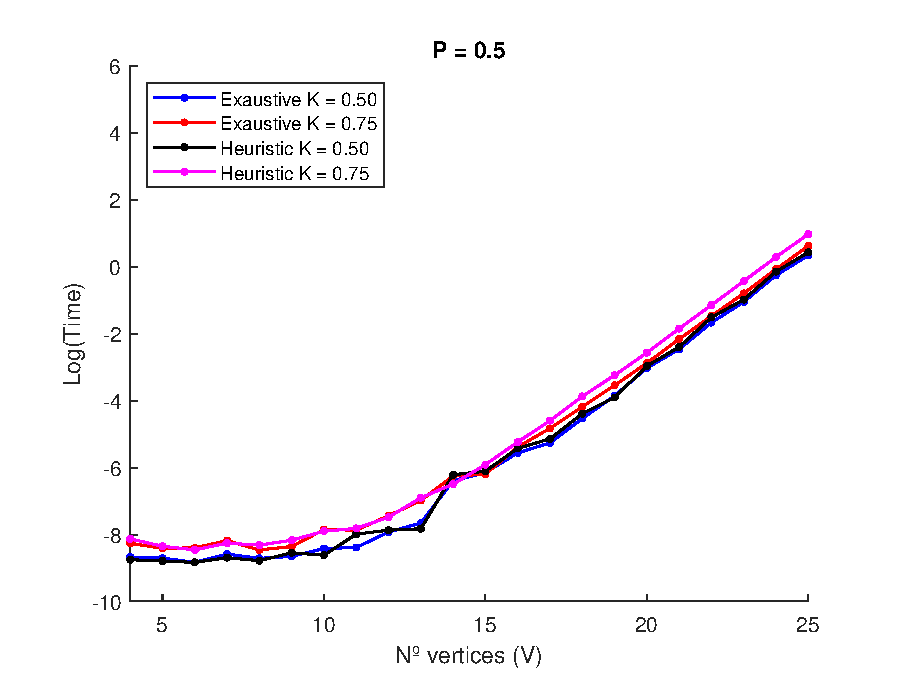
\includegraphics[scale = 0.5]{Figs/2_P050.eps}
\caption{Logaritmo do tempo de execução dos algoritmos em função do número de vértices - $P = 0.50$ - $K = 0.50, 0.75$}
\label{2_P050}
\end{figure}

\begin{figure}[h!]
\centering
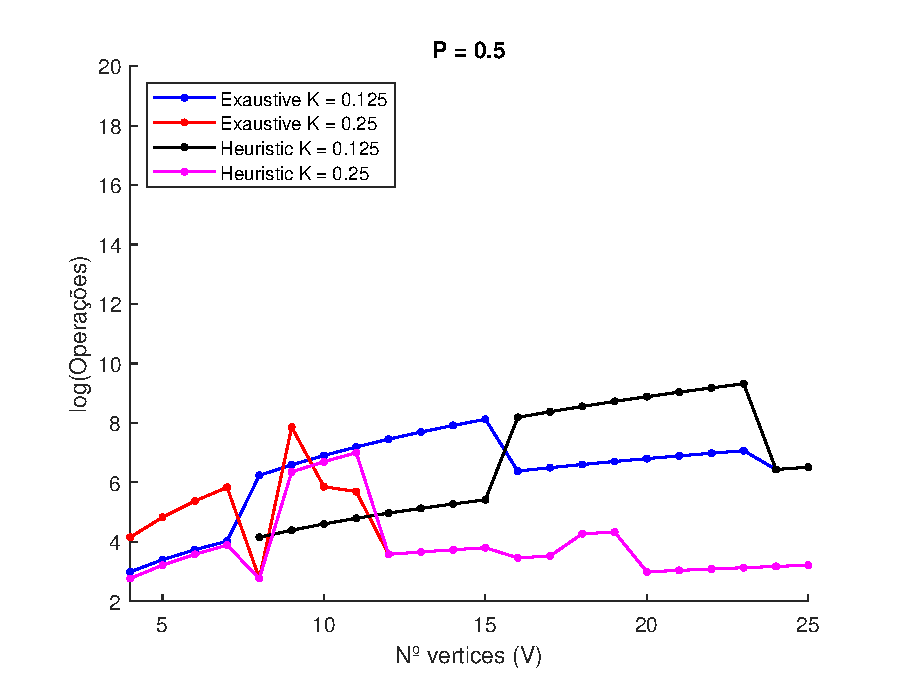
\includegraphics[scale = 0.5]{Figs/3_P050.eps}
\caption{Logaritmo do número de operações realizadas pelos algoritmos em função do número de vértices - $P = 0.50$ - $K = 0.125, 0.25$}
\label{3_P050}
\end{figure}

\begin{figure}[h!]
\centering
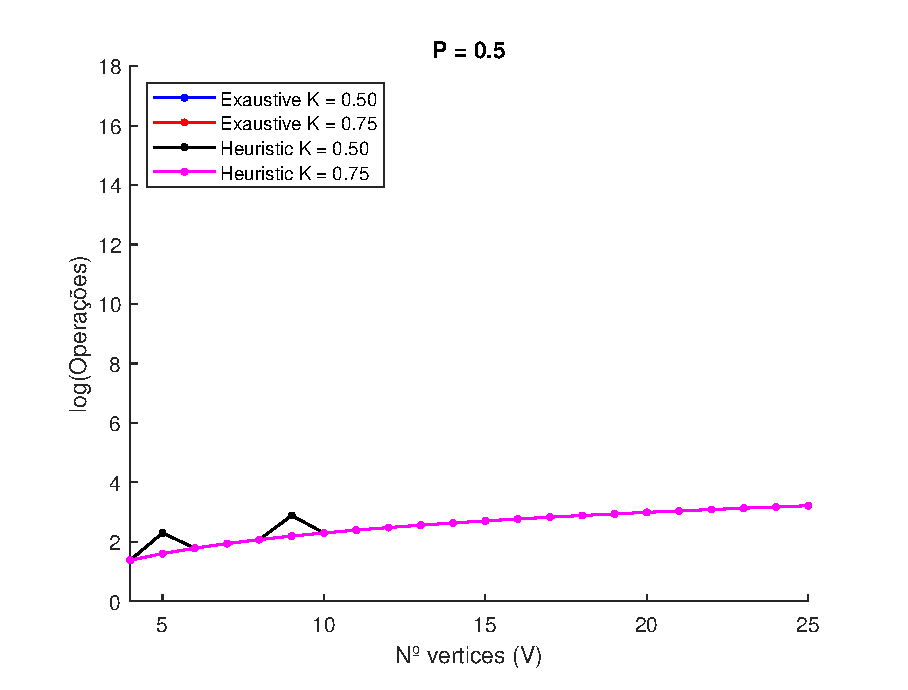
\includegraphics[scale = 0.5]{Figs/4_P050.eps}
\caption{Logaritmo do número de operações realizadas pelos algoritmos em função do número de vértices - $P = 0.50$ - $K = 0.50, 0.75$}
\label{4_P050}
\end{figure}


\begin{figure}[h!]
\centering
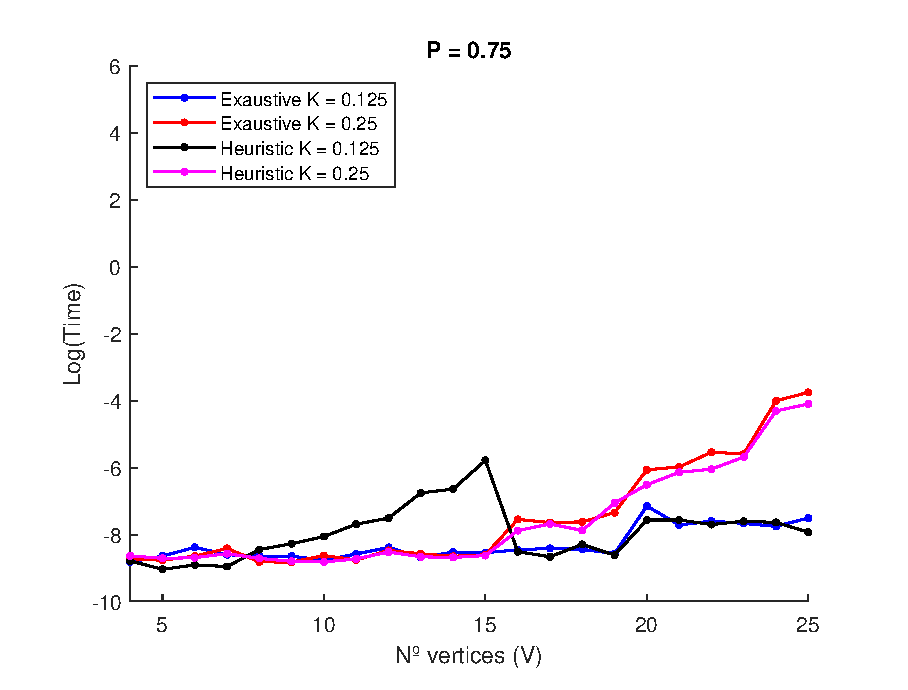
\includegraphics[scale = 0.5]{Figs/1_P075.eps}
\caption{Logaritmo do tempo de execução dos algoritmos em função do número de vértices - $P = 0.75$ - $K = 0.125, 0.25$}
\label{1_P075}
\end{figure}

\begin{figure}[h!]
\centering
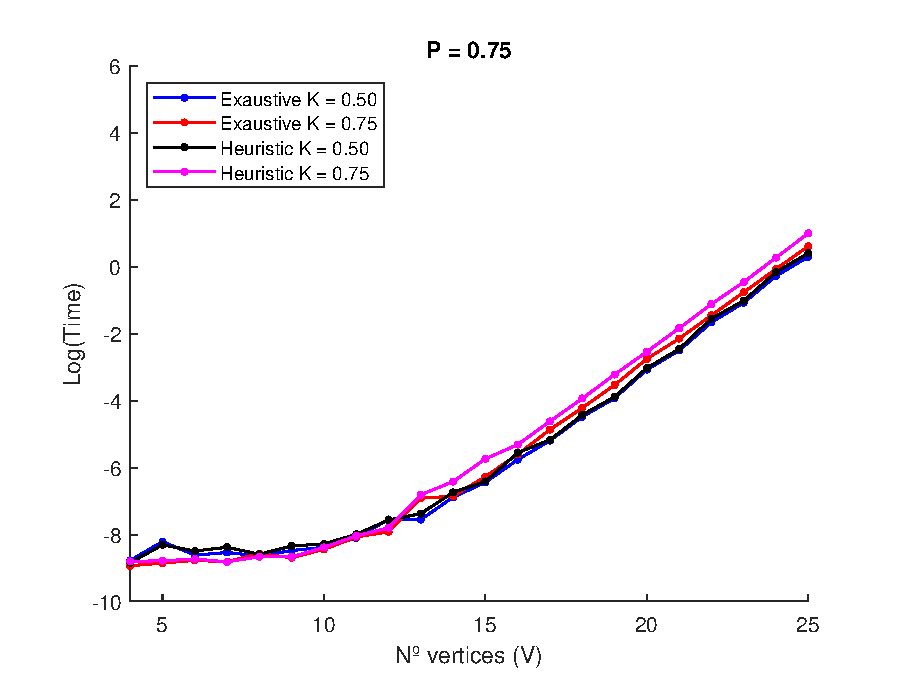
\includegraphics[scale = 0.5]{Figs/2_P075.eps}
\caption{Logaritmo do tempo de execução dos algoritmos em função do número de vértices - $P = 0.75$ - $K = 0.50, 0.75$}
\label{2_P075}
\end{figure}

\begin{figure}[h!]
\centering
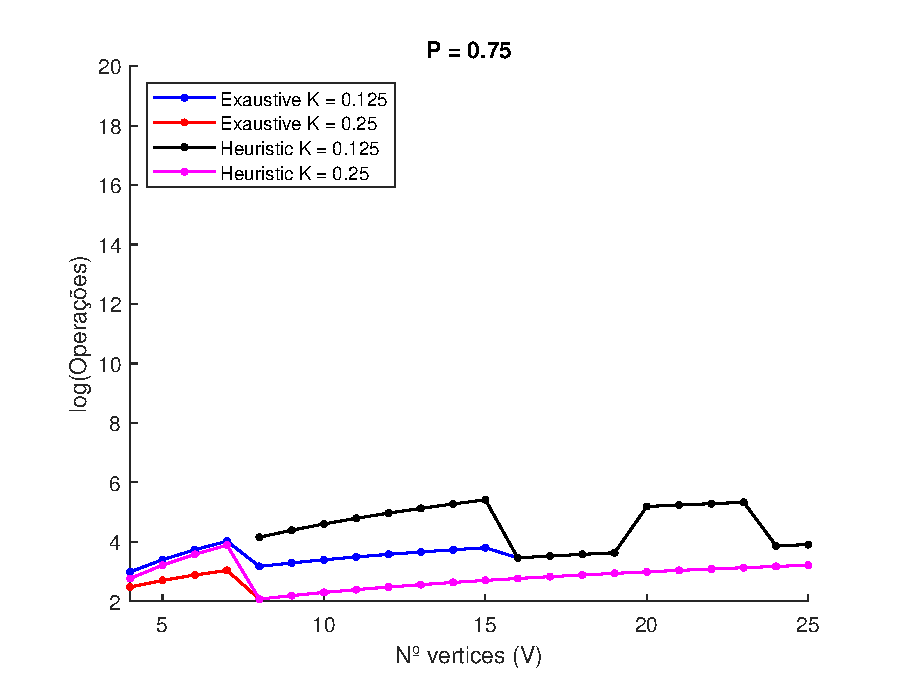
\includegraphics[scale = 0.5]{Figs/3_P075.eps}
\caption{Logaritmo do número de operações realizadas pelos algoritmos em função do número de vértices - $P = 0.75$ - $K = 0.125, 0.25$}
\label{3_P075}
\end{figure}

\begin{figure}[h!]
\centering
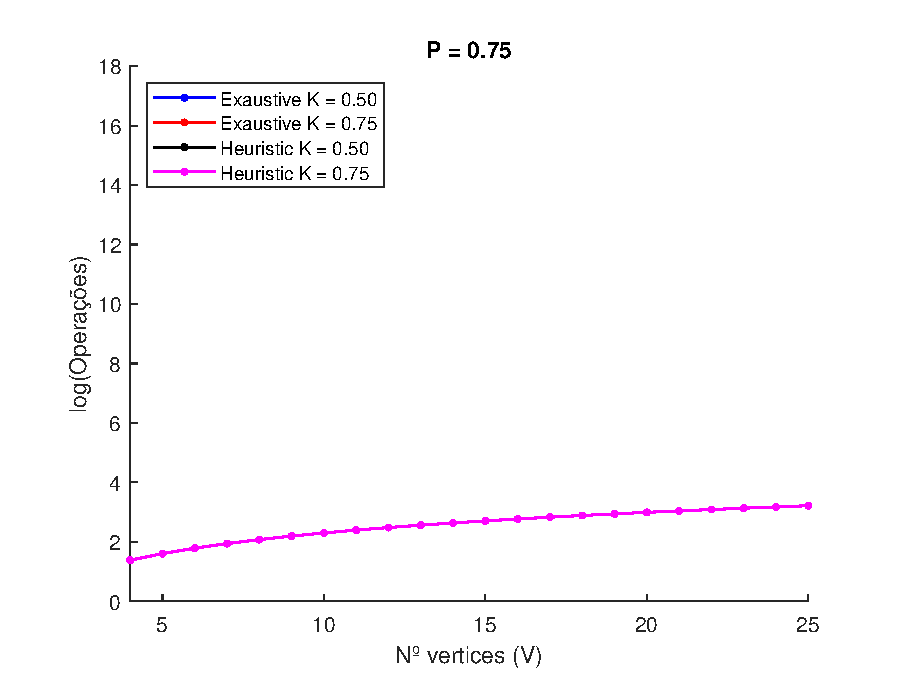
\includegraphics[scale = 0.5]{Figs/4_P075.eps}
\caption{Logaritmo do número de operações realizadas pelos algoritmos em função do número de vértices - $P = 0.75$ - $K = 0.50, 0.75$}
\label{4_P075}
\end{figure}

\clearpage
\section{Soluções}
\label{App_Solut}

Dado um par $(K,P)$ o/s vértice/s em que os algoritmos encontram solução, $V \in [4,5,...,30]$

\subsection{$P = 0.125$}

\subsubsection{$K = 0.125$}
Nenhuma solução encontrada para ambos os algoritmos.

\subsubsection{$K = 0.25$}
Nenhuma solução encontrada para o algoritmo Heurístico.

Solução Exaustiva: $V = [28,29]$

\subsubsection{$K = 0.50$}
Solução Heurística e Exaustiva: $V = [10,11,12,...,30]$

\subsubsection{$K = 0.75$}
Solução Heurística e Exaustiva: $V = [7,8,9,...,30]$

\subsection{$P = 0.25$}

\subsubsection{$K = 0.125$}
Nenhuma solução encontrada para ambos os algoritmos.

\subsubsection{$K = 0.25$}
Solução Heurística e Exaustiva: $V = [16,17,18,...,22,24,25,...,30]$
\subsubsection{$K = 0.50$}
Solução Heurística e Exaustiva: $V = [7,8,9,...,30]$

\subsubsection{$K = 0.75$}
Solução Heurística: $V = [7,8,9,...,30]$

Solução Exaustiva: $V = [6,7,8,...,30]$

\subsection{$P = 0.50$}

\subsubsection{$K = 0.125$}
Solução Heurística: $V = [24,25,26,...,30]$

Solução Exaustiva: $V = [16,17,18,...,30]$

\subsubsection{$K = 0.25$}
Solução Heurística: $V = [8,10,11,12,...,30]$

Solução Exaustiva: $V = [8,12,13,14,...,30]$

\subsubsection{$K = 0.50$}
Solução Heurística e Exaustiva: $V = [4,5,6,...,30]$

\subsubsection{$K = 0.75$}
Solução Heurística e Exaustiva: $V = [4,5,6,...,30]$

\subsection{$P = 0.75$}
\subsubsection{$K = 0.125$}
Solução Heurística: $V = [16,17,18,...,30]$

Solução Exaustiva: $V = [8,10,11,12,...,30]$

\subsubsection{$K = 0.25$}
Solução Heurística: $V = [8,10,11,12,...,30]$

Solução Exaustiva: $V = [4,5,6,...,30]$

\subsubsection{$K = 0.50$}
Solução Heurística e Exaustiva: $V = [4,5,6,...,30]$

\subsubsection{$K = 0.75$}
Solução Heurística e Exaustiva: $V = [4,5,6,...,30]$








\end{document}
